\section{Methodik}
\label{sec:Methodik}

% Ziel: 3-4 Seiten
% Ansatz: Aktionsforschung (Action Research)
% Quellen: Lewin, Susman & Evered, Reason & Bradbury, Mayring
% FOKUS: WIE/WARUM/Vorgehen, NICHT WAS/Ergebnisse

Dieses Kapitel erläutert das methodische Vorgehen zur Entwicklung der Drei-Artefakte-Architektur und des Master Creators. Im Zentrum steht die Frage, \textit{wie} und \textit{warum} die gewählten Methoden zur Lösung der in Kapitel~\ref{sec:IstAnalyse} identifizierten Probleme geeignet sind. Die detaillierten Ergebnisse werden in späteren Kapiteln ausgeführt werden.


\subsection{Aktionsforschung als methodischer Ansatz}
\label{subsec:Aktionsforschung}

Die vorliegende Arbeit folgt dem Paradigma der Aktionsforschung (Action Research) nach \cite{lewin:action_research1946}. Dieser Ansatz verbindet praktische Problemlösung mit wissenschaftlicher Erkenntnisgewinnung und eignet sich besonders für Kontexte, in denen der Forscher aktiv in das Untersuchungsfeld eingebettet ist \citep{reason:handbook_action_research2001}.

\subsubsection{Begründung der Methodenwahl}
\label{subsubsec:BegruendungMethode}

Die Wahl von Action Research wird durch vier kontextspezifische Faktoren begründet:

\begin{enumerate}
    \item \textbf{Instabilität des Zielsystems:} GRACE befindet sich in der Pilotphase mit kontinuierlich evolvierenden Datenstrukturen und JSON-Schemata. Klassische Erhebungsmethoden würden veraltete Zustände dokumentieren, während das System parallel weiterentwickelt wird. Action Research begreift die dynamische Veränderung des Forschungsgegenstandes nicht als Hindernis, sondern als konstitutiven Bestandteil der Methode. Die Entwicklung der vorgestellten Artefakte erstreckte sich über einen Zeitraum von drei Monaten. Multiple Iterationen, sogenannte \textit{Action Research Cycles}, wurden durchlaufen, um sich an die dynamischen Veränderungen anzupassen. Das Phänomen der dynamischen Veränderung des Analyseobjekts wird in der Literatur als \textit{Moving Target}-Effekt bezeichnet wird.

    \item \textbf{Fragmentiertes Wissen als Kernproblem:} Das interne Konfigurationswissen existiert verteilt über Azure DevOps Backlogs, E-Mail-Korrespondenzen, Git-Historien und informelle Teamgesprächen. Das externe Konfigurationswissen liegt häufig in ähnlich fragmentierter Form beim Kunden. Es fehlt eine zentrale, strukturierte Wissensbasis. Das SECI-Modell nach \cite{nonaka:knowledge_creating_company1995} adressiert dieses Problem durch systematische Externalisierung: Die Drei-Artefakte-Architektur überführt dieses fragmentierte Wissen in explizite, maschinenlesbare Formate.

    \item \textbf{Impraktikabilität formaler SME-Interviews:} Das Konfigurationsteam umfasst 5 Personen mit vollem Projektgeschäft während der Pilotphase. Mehrstündige, strukturierte Experteninterviews würden operative Kapazitäten überlasten. Regelmäßige informelle Gespräche während der täglichen Arbeit ermöglichen hingegen kontinuierliche Wissenserfassung ohne zusätzlichen Zeitaufwand. \cite{jackson:par2010} validiert diesen Ansatz: In einer vergleichbaren Studie zur Wissensexternalisierung bei Ressourcenknappheit erwies sich partizipative Aktionsforschung als praktikable Alternative zu formalen Interviewmethoden.

    \item \textbf{Eingebettete Forscherrolle:} Der Autor ist selbst Teil des Konfigurationsteams und hat direkten Zugang zu Prozessen, Werkzeugen und implizitem Wissen. Diese Position ermöglicht teilnehmende Beobachtung und iterative Verfeinerung der entwickelten Artefakte. \cite{susman:action_research1983} argumentieren, dass Action Research besonders dann geeignet ist, wenn eine Distanzierung des Forschers vom Untersuchungsfeld nicht möglich oder nicht sinnvoll ist, eine Bedingung, die im vorliegenden Kontext erfüllt ist.

    \item \textbf{Quantifizierbare Problemstellungen:} Die in Kapitel~\ref{sec:IstAnalyse} identifizierten Probleme manifestieren sich in messbaren Größen (Fehlerrate, Vollständigkeit, Reproduzierbarkeit, Zeit), was eine empirische Validierung der entwickelten Artefakte durch kontrolliertes Experiment ermöglicht. Action Research kombiniert praktische Problemlösung mit wissenschaftlicher Evaluation dieser Lösungen.
\end{enumerate}


\subsection{Forschungszyklus und Iterationen}
\label{subsec:Forschungszyklus}

Der Action-Research-Zyklus (Plan $\rightarrow$ Act $\rightarrow$ Observe $\rightarrow$ Reflect) wurde in dieser Arbeit über mehrere Iterationen operationalisiert und manifestiert sich auf multiple Arten und Weisen. Auch bei der Gliederung dieser Arbeit zeichnet sich die Action Research Methode ab, dabei ist die Ist-Analyse und die Methodik der Plan-Zyklus, die Implementierung der Act-Zyklus und die Ergebnisse der Observe-Zyklus mit Einleitung des Reflect-Zyklusses, der im Fazit und Ausblick vervollständigt wird. Die gesamte Entwicklung erstreckte sich über einen Zeitraum von drei Monaten zuzüglich zwei Wochen krankheitsbedingter Unterbrechung. Innerhalb der Entwicklung lässt sich das Muster ebenso betrachten, sogar bei den granularsten Einheiten. Die folgende Darstellung gliedert die Entwicklung in die typischen fünf Phasen sequenziell sortiert, wobei jede Phase multiple Artefakte parallel hervorbrachte. Daraufhin wird die Vorgehensweise in den jeweiligen Phasen erklärt.

\begin{figure}[htbp]
    \centering
    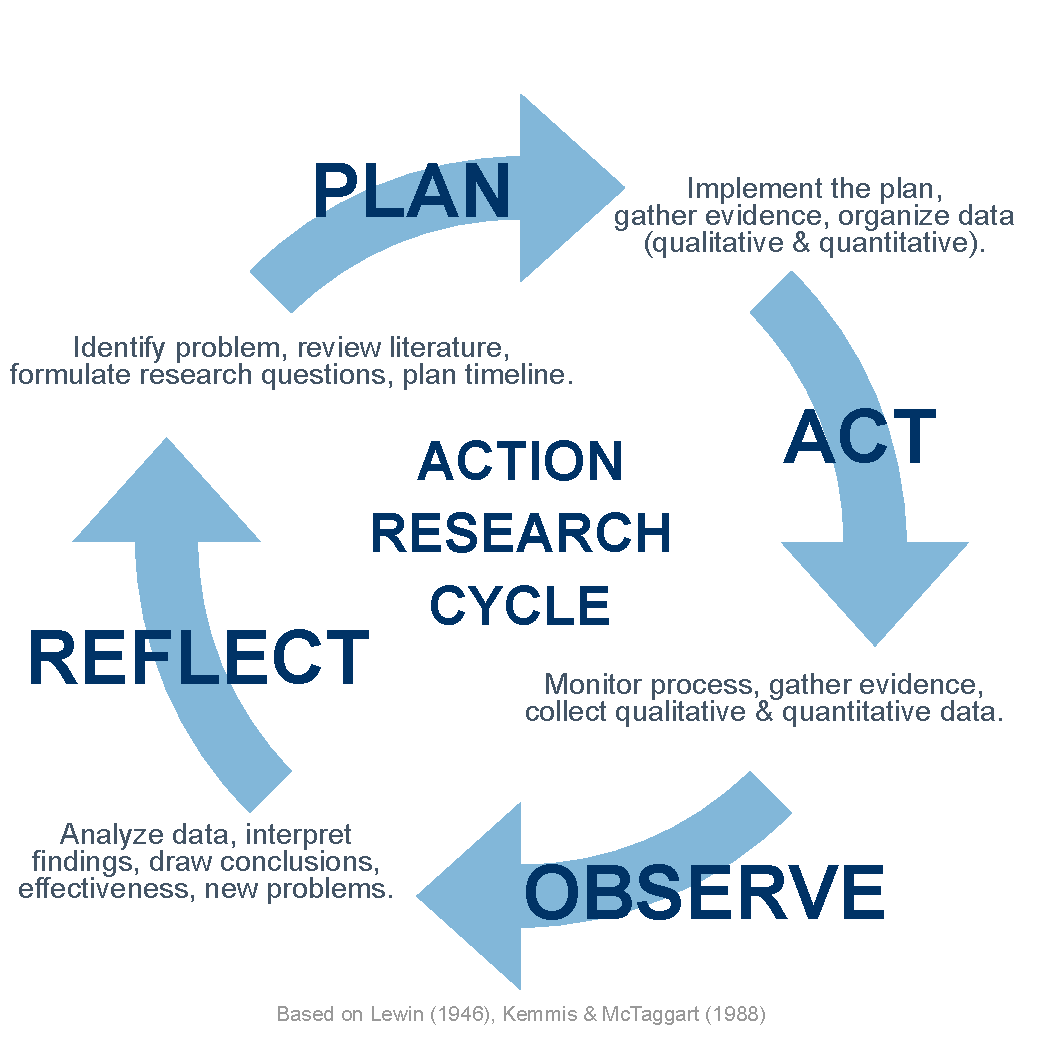
\includegraphics[width=0.8\textwidth]{@Bilder/ActionResearchCycle.pdf}
    \caption{Action Research Zyklus nach Lewin (1946): Iterative Phasen von Planung, Handlung, Beobachtung und Reflexion - Quelle: [Topić 2026]}
    \label{fig:ActionResearchCycle}
\end{figure} 


\subsubsection{Phase 0: Demo-Werk-Entwicklung als Erkenntnisfundament}
\label{subsubsec:Phase0}

Parallel zur Problemanalyse bestand eine praktische Aufgabenstellung (\textbf{Plan}): Die Entwicklung eines Demo-Werks zur Präsentation der GRACE-Fähigkeiten auf der EC Conference Digitalisation. Dieses Praxisprojekt erfüllte methodisch eine duale Funktion: Einerseits diente es als Showcasing-Tool für Kundenakquise, andererseits fungierte es als empirische Grundlage für die systematische Erfassung der GRACE-Konfigurations-anforderungen.

\paragraph{Methodische Besonderheit: Learning by Doing}

Die Demo-Werk-Entwicklung folgte keinem vorab definierten Prozessmodell, sondern erfolgte explorativ (\textbf{Act}) durch \glqq Code as Documentation\grqq{}-Ansatz: Reverse Engineering bestehender JSON-Exporte, Trial-and-Error bei der Konfiguration, und iterative Fehlerkorrektur. Diese methodische Besonderheit entspricht dem Action-Research-Prinzip nach \cite{lewin:action_research1946}: Problemlösung und Erkenntnisgewinnung sind iterativ verzahnt.

\paragraph{Domänenauswahl: Farb- und Lackproduktion}

Die Wahl der Produktionsdomäne (Pigmentpaste-Produktion) wurde durch vier Faktoren begründet:

\begin{enumerate}
    \item \textbf{Zielgruppe der EC Conference:} Fachpublikum aus der Lack- und Farbenindustrie
    \item \textbf{Verfügbare Fachliteratur:} Umfangreiche technische Dokumentation ermöglichte fundierte Modellierung ohne Kundendaten
    \item \textbf{Domänenexperte im Team:} Ehemaliger Maschinenführer mit Praxiserfahrung validierte Plausibilität
    \item \textbf{GRACE-Feature-Validierung:} Komplexe Prozessabhängigkeiten (Reinigungszyklen, mengenabhängige Zeitberechnungen) eigneten sich zur Validierung von Properties und Formelausdrücken
\end{enumerate}

\paragraph{Wissensquellen und Systematik}

Die Entwicklung folgte einer systematischen Wissensintegration aus drei Quellen:

\begin{itemize}
    \item \textbf{Fachliteratur:} Branchenstandards für Materialklassen, Maschinentypen, Prozessabläufe und Zeitberechnungsmethoden \citep{vci:lacke_farben2018, mueller:lackformulierung2017, goldschmidt:lackproduktion2019, REFA2012}
    \item \textbf{Domänenexpertise:} Praxiserfahrung des Maschinenführers validierte Plausibilität und lieferte Erfahrungswerte \citep{grace:fragensammlung_maschine2025}
    \item \textbf{GRACE-Anforderungen:} Bewusste Integration komplexer Features (mengenabhängige Zeitfunktionen, Property-basierte Materialzuordnung, verschachtelte Referenzstrukturen) zur späteren Validierung der Konfigurationslogik
\end{itemize}

\paragraph{Methodische Reflektion}

Die während dieser Phase durchgeführte Reverse-Engineering-Analyse offenbarte zentrale Erkenntnisse (\textbf{Observe}): (1) die Abhängigkeitskette zwischen den sechs Entitätstypen, (2) ID-Konsistenz als kritischer Erfolgsfaktor und (3) die Komplexität verschachtelter Referenzstrukturen bei Recipes. Die \textbf{Reflexion} dieser Beobachtungen führte zur Erkenntnis, dass das fragmentierte Konfigurationswissen systematisch externalisiert werden muss (\textbf{Reflect}). Diese Erkenntnisse bildeten die Basis für das Entity Mapping Workbook (Phase~1) und die 6-Punkte-Validierungscheckliste. Die konkreten technischen Details des Demo-Werks werden in Kapitel~\ref{sec:Implementation} dokumentiert.


\subsubsection{Phase 1: Wissensexternalisierung durch Entity Mapping und Validierung}
\label{subsubsec:Phase1}

Basierend auf den Erkenntnissen der Demo-Werk-Entwicklung (\textbf{Plan}) wurden in dieser Phase zwei zentrale Artefakte zur Wissensexternalisierung entwickelt (\textbf{Act}).
\\\\
Das \textbf{Entity Mapping Workbook} soll dem Problem der \textbf{Fragmentierung des Konfigurationswissens} dienen, indem es das über verschiedene Quellen verteilte implizite Wissen in eine zentrale, formale Struktur externalisiert. Gleichzeitig soll es durch Definition einheitlicher JSON-Schemata und Validierungsregeln dem Problem der \textbf{fehlenden Standardisierung} entgegenwirken.

\noindent Die Entwicklung erfolgte nach der qualitativen Inhaltsanalyse \citep{mayring:qualitative2015}: Multiple Datenquellen wurden systematisch analysiert und zu allgemeinen ER-Kardinalitäten abstrahiert, um Overfitting auf einzelne Datensätze zu vermeiden. Die zentrale Herausforderung bestand darin, multi-direktionale Beziehungen mit Versionierung korrekt abzubilden.
\\\\
Parallel wurde eine \textbf{6-Punkte-Validierungscheckliste} entwickelt, die ebenso dem Problem der \textbf{fehlenden Standardisierung} dienen soll, indem sie einheitliche Qualitätskriterien für Konfigurationen definiert. Die Checkliste systematisiert empirisch beobachtete Fehlertypen. Die konkreten Validierungsregeln werden in Kapitel~\ref{sec:Implementation} dokumentiert.

\paragraph{Methodische Reflektion}

Die Checkliste dient als explizites Werkzeug zur Qualitätssicherung (\textbf{Observe}) und wird in Kapitel~\ref{sec:Evaluation} zur Messung der Konfigurationsqualität verwendet. Die \textbf{Reflexion} ergab, dass die Kombination aus strukturierter Schema-Doku-mentation und operationalisierten Validierungsregeln die konzeptuelle Basis für LLM-gestützte Automatisierung bildet (\textbf{Reflect}). Diese Erkenntnis motivierte den Übergang zur Tool-Entwicklung in Phase~2.

\subsubsection{Phase 2: Initiales Prototyping und gescheiterte Monolith-Ansätze}
\label{subsubsec:Phase2}

Diese Phase umfasste das initiale Prototyping zur LLM-gestützten Entitätsgenerierung (\textbf{Plan}). Die Prompts wurden nach den Prinzipien des Reverse Prompting aufgebaut, jedoch mit einer methodischen Verfeinerung. Das Modell sollte nicht einfach einen Prompt erstellen, um die analysierte Datengrundlage zu reproduzieren, sondern es wurde um ein Vorgehen erweitert, welches durch die Entwicklung von Sora AI für Android inspiriert war \citep{openai:sora_android2025}. Nach der Analyse im Reverse Prompting-Vorgehen werden mehrere Schritte zwischengeschoben. Die Annahmen des LLMs aus der Analyse werden vom Instrukteur zusätzlich analysiert. Die Trugschlüsse werden korrigiert und zurück an das LLM übermittelt. Erst dann wird das Modell angewiesen einen Prompt zu generieren, die das Ergebnis reproduziert. Diese Vorgehensweise wird wiederholt, bis das LLM richtige Ergebnisse erzielt. So wurde die Logik des Master Creators stetig verbessert. Eine feine Änderung, die die Qualität der Ergebnisse iterativ steigern kann, aber dazu mehr in Kapitel~ \ref{sec:Implementation}, um nicht zu viel vorzugreifen. 

\paragraph{Monolithischer Prompt-Ansatz}

Der verfolgte Ansatz (\textbf{Act}) nutzte einen umfänglichen Prompt, der alle Abhängigkeiten zwischen den sechs Entitätstypen direkt abbilden sollte. Das Ziel war, in einem einzigen LLM-Aufruf eine vollständige GRACE-Konfiguration zu generieren.

\paragraph{Methodische Reflektion}

Dieser Ansatz funktionierte zu diesem Zeitpunkt nicht (\textbf{Ob-serve}). Die \textbf{Reflexion} ergab, dass die Komplexität der verschachtelten Abhängigkeiten (insbesondere Recipe-Verknüpfungen mit Material-BOM-Process-Referenzen) die Kapazität eines einzelnen Prompt-Kontexts übersteigt (\textbf{Reflect}). Die hohe Fehlerrate bei Referenzauflösungen motivierte den strategischen Wechsel zu einem modularen Ansatz, ebenso inspiriert nach \cite{openai:sora_android2025}.

\subsubsection{Phase 3: Blueprint-Prinzip und modulare Einzelcreatoren}
\label{subsubsec:Phase3}

Als Reaktion auf die Limitationen der monolithischen Ansätze (\textbf{Plan}) wurde in dieser Phase ein modularer Entwicklungsansatz verfolgt (\textbf{Act}).
\\\\
Das \textbf{Blueprint-Prinzip} basiert auf der schrittweisen Entwicklung: Ein einfaches Modul für einen einzelnen Entitätstyp wurde entwickelt und validiert. Dieses Grundprinzip wurde anschließend systematisch auf alle weiteren Entitätstypen übertragen.

\paragraph{Modularer Ansatz und Rückintegration}

Der Ansatz verfolgte zunächst eine schrittweise Spezialisierung: Ein einzelner Entitätstyp wurde isoliert betrachtet, dessen Generierungslogik entwickelt und validiert. Dieses Prinzip wurde systematisch auf alle sechs Entitätstypen übertragen. Nach erfolgreicher Validierung der Einzelmodule wurden die modularen Erkenntnisse wieder in eine zusammenhängende Prompt-Struktur integriert.

\paragraph{Methodische Reflektion}

Der modulare Ansatz ermöglichte kontrollierte Generierung mit reduzierten Fehlerquellen und validierte die Machbarkeit LLM-gestützter Entitätsgenerierung (\textbf{Observe}). Die \textbf{Reflexion} offenbarte jedoch neue Limitationen isolierter Module: fehlende Referenzauflösung zwischen Entitäten und mangelnde Session-Historie verhinderten die Erstellung vollständiger entitätsübergreifernder Beziehungen in den Konfigurationen (\textbf{Reflect}). Diese Erkenntnis motivierte die Rückintegration in ein unified System mit Session-Management in Phase~4.

\subsubsection{Phase 4: Master Creator mit Session-Management}
\label{subsubsec:Phase4}

Diese Phase integrierte die modularen Erkenntnisse aus Phase~3 (\textbf{Plan}) in ein einheitliches System mit intelligenter Referenzauflösung und Session-Persistenz (\textbf{Act}).

\paragraph{Integration und Session-Management}

Der \textbf{Master Creator} adressierte die Limitationen der Einzelcreatoren durch Integration aller sechs Entitätstypen in ein einheitliches Chat-Interface. Ein zentrales Session-Management ermöglichte die automatische Referenzauflösung zwischen abhängigen Entitäten (z.B. Recipe-Generierung basierend auf zuvor erstellten Materials, BOMs und Processes).

\paragraph{Automatisierung und Validierung}

Der Master Creator soll durch automatisierte Referenzauflösung und integrierte Validierung zur Reduktion der Fehlerrate, durch Zeitersparnis bei der Konfigurationserstellung und durch dokumentierte Chat-Konversationen zur Reproduzierbarkeit beitragen.

\paragraph{Iterative Verfeinerung}

Jede Iteration bildete einen Mikro-Zyklus: Fehlerbeobachtung durch praktische Anwendung (\textbf{Observe}), \textbf{Reflexion} der Fehlerursachen (\textbf{Reflect}), Prompt-Anpassung als neuer \textbf{Plan}, erneute Testung (\textbf{Act}). Die technische Evolution mit konkreten Fehlerquellen und Lösungsansätzen wird in Kapitel~\ref{sec:Implementation} dokumentiert.

\paragraph{Methodische Reflektion}

Die technische Umsetzung wird in Kapitel~\ref{sec:Implementation} detailliert beschrieben. Diese Phase markiert den Abschluss des Entwicklungs-Zyklus und den Übergang von fragmentiertem, manuellem Konfigurationswissen zu einem integrierten, LLM-gestützten Workflow.


\subsubsection{Ungeplante methodische Besonderheit: Datenverlust}
\label{subsubsec:NASCrashValidierung}

Während der Bearbeitungszeit ereignete sich ein Ausfall des Network Attached Storage (NAS) im Unternehmen, der zum Verlust von Demo-Konfigurationsdaten führte. Zusätzlich verhinderten Bugs in der GRACE-Exportfunktion den vollständigen Export bestimmter Entitäten (insbesondere Properties).

\noindent Dieses unerwartete Ereignis ermöglichte eine praxisnahe Validierung des Action-Research-Ansatzes. Die Rekonstruktion erfolgte iterativ unter Nutzung des Master Creators bis zur vollständigen Rekonstruktion \citep{grace:demo_werk_restored2026}.

\subsection{Datenauswertung}
\label{subsec:Datenauswertung}

Die erhobenen Daten wurden mittels verschiedener Auswertungsmethoden analysiert und in strukturierte Artefakte überführt. Die Auswertung erfolgte iterativ und orientierte sich an etablierten Methoden der qualitativen Forschung sowie der Skalenentwicklung.

\subsubsection{Qualitative Inhaltsanalyse für Entity Mapping}
\label{subsubsec:QualitativeInhaltsanalyse}

Die Entwicklung des Entity Mapping Workbooks erfolgte nach der qualitativen Inhaltsanalyse nach \cite{mayring:qualitative2015}. Die Methode umfasst drei Schritte:

\begin{enumerate}
    \item \textbf{Kodierung:} JSON-Exporte aus der Demo-Werk-Konfiguration \citep{grace:demo_werk_restored2026} und generische Beispiel-JSONs \citep{grace:jsons_example2025} wurden systematisch analysiert. Für jedes Entitätsfeld wurde eine Kodierregel erstellt (Definition, Ankerbeispiel, Abgrenzung).

    \item \textbf{Kategorisierung:} Wiederkehrende Muster (z.B. ID-Strukturen, Versionsattribute, Referenztypen) wurden zu allgemeinen Kategorien abstrahiert.

    \item \textbf{Verallgemeinerung:} Aus den spezifischen Datensätzen wurden generalisierbare JSON-Schemata abgeleitet, um Overfitting auf einzelne Konfigurationen zu vermeiden.
\end{enumerate}

\noindent Diese systematische Abstraktion stellte sicher, dass das Entity Mapping Workbook nicht auf ein spezifisches Demo-Werk zugeschnitten ist, sondern allgemeingültige Konfigurationsmuster dokumentiert.

\subsubsection{Fragebogenentwicklung nach DeVellis}
\label{subsubsec:Fragebogenentwicklung}

Der GRACE Onboarding Fragebogen wurde nach den Prinzipien der Skalenentwicklung von \cite{devellis:scale_development2017} entwickelt. Er wurde in den vorherigen Phasen nicht explizit erwähnt. Die Entwicklung folgt jedoch der gleichen iterativen Vorgehensweise nach Action Research, nur in einem separaten Loop. Über die Gliederung der Thesis lässt er sich wieder in einem gesamt Kontext der Action Research Methode überführen. Der Fragebogen soll dem Problem der \textbf{Fragmentierung} entgegenwirken. Indem er fragmentiertes Kundenwissen in ein standardisiertes Format überführt. Dies soll das Problem der \textbf{fehlenden Standardisierung} bei der Wissenserhebung lösen. Das Vorgehen umfasste:

\begin{enumerate}
      \item \textbf{Item-Generierung:} Sammlung potenzieller Fragen aus unzugänglichen Quellen (Azure DevOps Wikis, E-Mail-Korrespondenz,
      Git-Historie, interne Dokumente)\footnote{Abgeleitet aus internen Kundenprojekt-Daten (NDA-geschützt, nicht öffentlich
      hinterlegbar).} und zugänglichen Wissensquellen (Expertengespräche, persönliche Erfahrung aus Konfigurationsprojekten, APS-Interviewskript aus
      früherer akademischer Arbeit \citep{grace:interviewskript2024}, Gesprächstranskript zur Entwicklung des Fragenkatalogs \citep{grace:gespraechstranskript_fragenkatalog2025})

    \item \textbf{Redundanzeliminierung:} Identifikation und Zusammenführung von Fragen mit überlappenden Informationsgehalten.

    \item \textbf{Essenzialitätsprüfung:} Fokussierung auf Fragen, die notwendige (nicht optionale) Informationen erheben.

    \item \textbf{Praktikabilitätsanpassung:} Anpassung des Umfangs an zeitliche und ressourcenbezogene Rahmenbedingungen (Workshop-Dauer, Kundenkapazitäten).
\end{enumerate}

\noindent Weitere iterative Verfeinerungen erfolgten durch Anwendung in realen Kundenprojekten und anschließender Anpassung basierend auf Feedback.

\subsubsection{Reverse Engineering für JSON-Strukturen}
\label{subsubsec:ReverseEngineering}

Bestehende JSON-Konfigurationen wurden mittels Reverse Engineering und Reverse Prompting analysiert, um implizite Strukturregeln zu identifizieren:

\begin{itemize}
    \item \textbf{Strukturanalyse:} Feldtypen, Verschachtelungstiefe, optionale vs. obligatorische Felder
    \item \textbf{Abhängigkeitsanalyse:} Referenzbeziehungen zwischen Entitäten, Versionierungslogik
    \item \textbf{Validierungsregeln:} Implizite Constraints
\end{itemize}

\noindent Diese Analyse bildete die Grundlage für die 6-Punkte-Validierungscheckliste, die empirisch beobachtete Fehlerquellen systematisiert und in den System-Prompt und andere LLM-gerechte Artefakte aufgenommen wurde. Außerdem diente sie auch als Metrik im Evaluierungsexperiment mit dem Master Creator.

\subsubsection{Prozessmodellierung mit BPMN}
\label{subsubsec:Prozessmodellierung}

Die Konfigurationsprozesse wurden mittels Business Process Model and Notation (BPMN) dokumentiert. Die Entwicklung der Prozessmodelle erfolgte ebenso iterativ und parallel zur Artefaktentwicklung durch:

\begin{itemize}
    \item \textbf{Teilnehmende Beobachtung:} Direktes Shadowing von Konfigurationsschritten während der Demo-Werk-Entwicklung und realer Kundenprojekte
    \item \textbf{Zeitmessungen:} Erfassung der Durchlaufzeiten für einzelne Prozessschritte unter realen Arbeitsbedingungen
    \item \textbf{Dokumentenanalyse:} Analyse bestehender Prozessskizzen und Arbeitsanweisungen aus Präsentationsmaterialien \citep{seitcom:grace_start_praesentation2024, seitcom:grace_test_praesentation2024, seitcom:grace_pitch_deck2024, grace:onboarding2024, seitcom:grace_investor_pitch2024}
    \item \textbf{Retrospektive Modellierung:} Nach Abschluss der Tool-Entwicklung wurden die Prozessvarianten formal modelliert
\end{itemize}

\noindent Die Modellierung folgt der BPMN 2.0-Notation und bildet verschiedene Prozessvarianten ab, um die methodische Evolution des Konfigurationsansatzes zu dokumentieren. Die konkreten Prozessmodelle und deren Auswertung werden in Kapitel~\ref{sec:Evaluation} präsentiert.


\subsection{Drei-Artefakte-Architektur als methodisches Framework}
\label{subsec:DreiArtefakteArchitektur}

Die \textbf{Drei-Artefakte-Architektur} bildet das konzeptuelle Fundament der Externalisierung und operationalisiert das SECI-Modell nach \cite{nonaka:knowledge_creating_company1995}. Die Architektur transformiert implizites Domänenwissen in LLM-konsumierbare Strukturen und soll den in Kapitel~\ref{sec:IstAnalyse} identifizierten Problemfeldern wie folgt dienen:

\begin{enumerate}
    \item \textbf{GRACE Onboarding Fragebogen:} Systematische Wissenserhebung beim Kunden, externalisiert implizites Produktionswissen in strukturierte Antworten. Soll der Vollständigkeit dienen, indem ein standardisiertes Maß für benötigte Informationen definiert wird.

    \item \textbf{Entity Mapping Workbook:} Formale JSON-Schemata mit Kardinalitäten und Validierungsregeln, externalisiert implizites Konfigurationswissen des Teams. Soll durch systematische Dokumentation der Abhängigkeiten zur Reduktion von Referenzfehlern und zur Standardisierung beitragen.

    \item \textbf{Standard Operating Procedures (SOPs):} Prozessdokumentation für Workshop (SOP 01), Tool-Nutzung (SOP 02) und Import (SOP 03), externalisiert implizites Prozesswissen. Soll der Reproduzierbarkeit dienen, indem Wissensträgerabhängigkeit durch dokumentierte Prozesse reduziert wird.
\end{enumerate}

\noindent Diese drei Artefakte entwickelten sich parallel zur technischen Tool-Entwicklung. Die gegenseitige Beeinflussung und iterative Verfeinerung dieser Artefakte wird in Kapitel~\ref{sec:Implementation} detailliert beschrieben.


\subsection{Technische Infrastruktur und Datenhoheit}
\label{subsec:TechnischeInfrastruktur}

Die technische Infrastruktur musste zwei widersprüchliche Anforderungen vereinen: LLM-basierte Automatisierung einerseits, absolute Datenhoheit andererseits. Kundenkonfigurationen enthalten sensible Produktionsdaten (Rezepturen, Kapazitäten, Schichtpläne), die unter DSGVO-Anforderungen und NDA-Verpflichtungen stehen. Cloud-basierte LLM-Lösungen (GPT-4, Claude) scheiden daher aus Compliance-Gründen aus.

\paragraph{Strategische Entscheidung}

Die Lösung bestand in einem \textbf{lokalen LLM-Deployment}, das alle Datenverarbeitung on-premise durchführt. Diese Architekturentscheidung erzwingt jedoch einen fundamentalen Trade-off: Kleinere Sprachmodelle (7B-Parameter-Klasse) sind mit verfügbarer Standard-Hardware betreibbar, erreichen aber nicht die Leistungsfähigkeit cloud-basierter Großmodelle (70B+ Parameter).

\noindent Dieser Trade-off wurde bewusst zugunsten der Datensouveränität entschieden. Die resultierende Vollständigkeit von 90-95\% (gegenüber potenziell 98\%+ bei Großmodellen) wurde als akzeptabel bewertet, da:

\begin{itemize}
    \item Privacy-Compliance nicht verhandelbar ist (rechtliche Anforderung)
    \item 90-95\% Vollständigkeit bereits eine signifikante Verbesserung gegenüber dem Status quo (60-70\%) darstellt
    \item Manuelle Nachbearbeitung der verbleibenden 5-10\% deutlich schneller ist als vollständige Neuerstellung
\end{itemize}

\noindent Die konkrete technische Umsetzung dieser strategischen Entscheidung (Modellauswahl, Deployment-Architektur, Validierungsmechanismen) wird in Kapitel~\ref{sec:Implementation} detailliert beschrieben.

\subsection{Evaluationsdesign quantitativer Probleme}
\label{subsec:Evaluationsdesign}

Die Evaluation der quantitativen Probleme adressiert die in Kapitel~\ref{sec:IstAnalyse} identifizierten Problemfelder durch ein kontrolliertes Experiment. Dieser Teil der Evaluation dient als Hauptteil der Evaluation, weil alle 5 Problemfelder gleichzeitig analysiert werden. Die quantitativen Probleme werden wie folgt operationalisiert:

\begin{itemize}
    \item \textbf{Fragmentierung und fehlende Standardisierung:} Messung über Vollständigkeitsgrad und Fehlerrate gemäß 6-Punkte-Checkliste
    \item \textbf{Wissensträgerabhängigkeit:} Messung über Reproduzierbarkeit durch drei unabhängige Probanden
    \item \textbf{Zeiteffizienz:} Messung der Konfigurationsdauer als Primärmetrik
    \item \textbf{Datenhoheit:} Adressiert durch technische Infrastruktur (lokales LLM-Deployment)
\end{itemize}

\noindent Die Evaluation kombiniert gemessene Praxisdaten mit einem kontrollierten Experiment. Die in den BPMN-Diagrammen (v1a, v1b) dargestellten Durchlaufzeiten basieren auf realen Konfigurationsprojekten.

\subsubsection{Kontrolliertes Validierungsexperiment}
\label{subsubsec:Experiment}

Zur Validierung der Tool-Effektivität wurde ein Within-Subjects-Experiment durchgeführt. Die Wahl dieses Designs folgt der Empfehlung von \cite{Doering2023} aus dem Inventar der Human- und Sozialwissenschaften zur Kontrolle menschlicher Störfaktoren. Die Fehlervarianz sollen durch interindividuelle Unterschiede minimiert werden und so die Effekte der Intervention des Master Creators präziser zu isolieren. Counterbalancing soll sequenzielle Effekte minimieren \citep{Doering2023}:\\

\noindent \textbf{Setup}
\\ 
Fiktive Produktkonfiguration mit standardisierter Komplexität: 5 Materialien, 5 Maschinen, 1 Produkt, 1 Prozess (mehrere Schritte), 1 BOM, 1 Rezept.

\paragraph{Bedingungen}
\begin{description}
    \item[Bedingung A (Baseline):] Manuelle Eingabe in GRACE UI ohne Hilfsmittel
    \item[Bedingung B (Intervention):] Master Creator + JSON-Import in GRACE
\end{description}

\noindent Jeder Proband absolvierte 6 Durchläufe pro Bedingung (alternierend, counterbalanced). Die Reihenfolge wurde zwischen den Probanden variiert, um Reihenfolgeeffekte zu kontrollieren.

\paragraph{Probanden}
\begin{itemize}
    \item \textbf{Proband 1:} Konfigurationsteam-Mitglied mit GRACE-Erfahrung und Master-Creator-Erfahrung
    \item \textbf{Proband 2:} Konfigurationsteam-Mitglied mit GRACE-Erfahrung, ohne Master-Creator-Erfahrung
    \item \textbf{Proband 3:} Konfigurationsteam-Mitglied mit GRACE-Erfahrung, ohne Master-Creator-Erfahrung
\end{itemize}

\paragraph{Metriken}
\begin{enumerate}
    \item \textbf{Zeit:} Dauer bis zur vollständigen Konfiguration (MM:SS,ms)
    \item \textbf{Fehlerrate:} Anzahl Validierungsfehler bei JSON-Import in GRACE
    \item \textbf{Checklisten-Vollständigkeit:} \\ Anzahl erfüllter Punkte der 6-Punkte-Validierungscheckliste ($v \in [0, 6]$)
\end{enumerate}

Die Ergebnisse dieses Experiments werden in Kapitel~\ref{sec:Evaluation} präsentiert.

\subsubsection{Statistische Auswertungsmethoden}
\label{subsubsec:StatistischeAuswertung}

Die quantitative Auswertung des kontrollierten Experiments erfolgt mittels deskriptiver Statistik. Für jede Bedingung (A: Baseline, B: Intervention) werden folgende Kennwerte nach \cite{Doering2023} berechnet:

\paragraph{Zeitreduktion (Primärmetrik)}

Die Konfigurationszeit $t$ wird in Sekunden erfasst. Für jede Bedingung wird der Mittelwert berechnet:

\[
\bar{t} = \frac{1}{n} \sum_{i=1}^{n} t_i
\]

Die Standardabweichung quantifiziert die Streuung der Messungen:

\[
s = \sqrt{\frac{1}{n-1} \sum_{i=1}^{n} (t_i - \bar{t})^2}
\]

Die prozentuale Zeitreduktion zwischen den Bedingungen wird berechnet als:

\[
\text{Reduktion} = \frac{\bar{t}_A - \bar{t}_B}{\bar{t}_A} \times 100\%
\]

\paragraph{Vollständigkeit und Fehlerrate}

Für jede Konfiguration wird die Anzahl erfüllter Validierungspunkte $v \in [0, 6]$ gemäß der 6-Punkte-Checkliste erfasst. Die durchschnittliche Vollständigkeit wird berechnet als:

\[
\bar{v} = \frac{1}{n} \sum_{i=1}^{n} v_i \quad \text{und} \quad \text{Vollständigkeit} = \frac{\bar{v}}{6} \times 100\%
\]

\noindent Fehler werden als diskrete Ereignisse gezählt. Der Mittelwert und die Standardabweichung der Fehleranzahl werden analog zur Zeitmetrik berechnet.

\paragraph{Reproduzierbarkeit}

Die Reproduzierbarkeit wird durch die Konsistenz der Ergebnisse über drei unabhängige Probanden gemessen. Für jede Metrik (Zeit, Vollständigkeit, Fehlerrate) wird die Inter-Proband-Variabilität über die Standardabweichung zwischen den Probanden-Mittelwerten quantifiziert.

\paragraph{Darstellung der Ergebnisse}

Die Ergebnisse werden in tabellarischer Form präsentiert:

\begin{itemize}
    \item \textbf{Zeit:} Mittelwert $\pm$ Standardabweichung (MM:SS $\pm$ SS)
    \item \textbf{Vollständigkeit:} Durchschnittliche Anzahl erfüllter Punkte und Prozentangabe
    \item \textbf{Fehlerrate:} Mittelwert $\pm$ Standardabweichung (Anzahl Fehler)
    \item \textbf{Reproduzierbarkeit:} Variabilität zwischen Probanden
\end{itemize}

\noindent Die statistischen Berechnungen erfolgen für $n = 6$ Durchläufe pro Proband und Bedingung. Die Ergebnisse werden in Kapitel~\ref{sec:Evaluation} präsentiert.

\subsubsection{Explorative Anwendung in der Praxis}
\label{subsubsec:ExplorativeAnwendung}

Parallel zum kontrollierten Experiment wurde der GRACE Onboarding Fragebogen und SOP~01 (Kundenworkshop durchführen) explorativ in zwei realen Kundenprojekten eingesetzt. Diese Anwendung erfolgte unter Produktionsbedingungen mit tatsächlichen Kundenanforderungen und diente primär der praktischen Erprobung der entwickelten Artefakte im Feldkontext.

\noindent Der Fragebogen wurde als Leitfaden zur strukturierten Wissenserhebung in initialen Kundenworkshops verwendet. Die erhobenen Informationen dienten als Eingabe für die nachgelagerte Konfigurationsentwicklung mit dem Master Creator. Diese explorative Anwendung ermöglichte qualitative Beobachtungen zur Praktikabilität der Artefakte, erhob jedoch keine quantitativen Vergleichsdaten. Die Erkenntnisse fließen als ergänzende qualitative Perspektive in Kapitel~\ref{sec:Evaluation} ein.

\subsubsection{Wissenschaftliche Gütekriterien des Experiments}
\label{subsubsec:Guetekriterien}

Das kontrollierte Validierungsexperiment wurde unter Berücksichtigung der wissenschaftlichen Gütekriterien Validität, Reliabilität und Objektivität konzipiert \citep{gothesis:methodikteil}.

\paragraph{Validität}

\begin{itemize}
    \item \textbf{Inhaltsvalidität:} Die 6-Punkte-Checkliste basiert auf empirisch beobachteten Fehlerquellen aus der Demo-Werk-Entwicklung und deckt kritische Validierungsaspekte ab (Vollständigkeit, ID-Konsistenz, Zeiteinheiten, BOM-Berechnung, Material-Referenzen, ID-Duplikate).

    \item \textbf{Konstruktvalidität:} Die gemessenen Dimensionen (Zeit, Vollständigkeit/Fehlerrate, Reproduzierbarkeit) operationalisieren das theoretische Konstrukt \glqq Konfigurationseffizienz\grqq{} entlang wissenschaftlich fundierter Dimensionen: Zeitwirtschaft nach REFA \citep{REFA2012}, Qualitätsmanagement (Fehlerreduktion) und Wissensmanagement (Reproduzierbarkeit durch Externalisierung).

    \item \textbf{Externe Validität:} Das standardisierte Experiment-Setup ermöglicht prinzipiell die Replikation durch andere Forschende. Die Übertragbarkeit auf andere APS-Kontexte ist durch die Domänenspezifität der Artefakte eingeschränkt, die methodische Vorgehensweise (Drei-Artefakte-Architektur) jedoch generalisierbar.
\end{itemize}

\paragraph{Reliabilität}

\begin{itemize}
    \item \textbf{Test-Retest-Reliabilität:} Jeder Proband absolvierte 6 Durchläufe pro Bedingung und System, was die Konsistenz der Messungen über mehrere Zeitpunkte hinweg ermöglicht.

    \item \textbf{Interrater-Reliabilität:} Reproduzierbarkeitstest durch drei unabhängige Probanden mit unterschiedlichen Master-Creator-Erfahrungsniveaus validiert, dass die entwickelten Artefakte (SOPs) von verschiedenen Personen konsistent angewendet werden können.

    \item \textbf{Methodische Kontrolle:} Counterbalanced Design reduziert Reihenfolgeeffekte; standardisiertes Experiment-Setup gewährleistet vergleichbare Bedingungen über alle Durchläufe hinweg.
\end{itemize}

\paragraph{Objektivität}

\begin{itemize}
    \item \textbf{Durchführungsobjektivität:} Standardisiertes Experiment-Setup mit klaren Anweisungen und identischen Aufgabenstellungen für alle Probanden minimiert Einflüsse durch unterschiedliche Versuchsbedingungen.

    \item \textbf{Auswertungsobjektivität:} Objektive Metriken (Zeit in MM:SS,ms, Anzahl erfüllter Checklisten-Punkte, Anzahl Fehler) minimieren Interpretationsspielräume bei der Datenauswertung.

    \item \textbf{Interpretationsobjektivität:} Die 6-Punkte-Checkliste definiert binäre Validierungskriterien (erfüllt/nicht erfüllt) ohne subjektive Bewertungsskalen. Die Einbeziehung von Probanden ohne Master-Creator-Vorerfahrung reduziert potenzielle Verzerrungen durch Entwicklernähe.
\end{itemize}

\noindent Die Kombination dieser Gütekriterien stellt sicher, dass die Evaluationsergebnisse des Experiments wissenschaftlich fundiert und nachvollziehbar sind.


\subsection{Limitierungen der Methodik}
\label{subsec:LimitierungenMethodik}

Die gewählte Methodik unterliegt spezifischen Einschränkungen:

\begin{enumerate}
    \item \textbf{Eingebettete Forscherrolle:} Der Autor ist Teil des Konfigurationsteams, was zu Bestätigungstendenz bei der Artefakt-Entwicklung führen kann. Dies wird durch Kollegenfeedback während der Entwicklung, objektive Metriken (Zeit, Vollständigkeit, Checklisten-Punkte etc.) und einem Experiment mit standardisierten Bedingungen mitigiert.

    \item \textbf{Overfitting-Prävention durch systematische Verallgemeinerung:} Das Demo-Werk wurde in Phase 0 dieser Arbeit entwickelt und bildete die empirische Grundlage für die in Phase 4 entwickelte Master-Creator-Automatisierung. Um Overfitting auf einen spezifischen Datensatz zu verhindern, erfolgte eine systematische Verallgemeinerung mehrerer Datenquellen (Restored\_JSONS, alte Demo-Werk-Fragmente, generische Example-JSONs) über abgewandeltes Reverse Prompting zu allgemeinen ER-Kardinalitäten und JSON-Schemata, die im Entity Mapping Workbook dokumentiert wurden \citep{mayring:qualitative2015}. Diese methodische Abstraktion stellt sicher, dass das Tool nicht auf die Besonderheiten eines einzelnen Projekts zugeschnitten ist, sondern generalisierbare Konfigurationsmuster verwendet.

    \item \textbf{GRACE-Instabilität während Pilotphase:} Die Pilotphase war durch technische Instabilität geprägt: JSON-Import-Bugs verhinderten die Nutzung bestimmter Features (Properties, Maschinenreferenzen in Prozessen), und Systemcrashes beeinträchtigten die Entwicklungsarbeit. Der Master Creator fokussiert daher auf die Kernkonfiguration (6 Entitätstypen ohne optionale Erweiterungen), um trotz dieser Rahmenbedingungen und des zusätzlichen Zeitdrucks durch den NAS-Crash den Zeitrahmen einzuhalten. Die Bugs wurden nach Abschluss der Master-Creator-Entwicklung behoben, eine nachträgliche Erweiterung war jedoch aus Zeitgründen nicht mehr möglich.
\end{enumerate}

\noindent Trotz dieser Limitierungen bietet die Action-Research-Methodik den Vorteil, der simultanen Entwicklung und Evaluierung praktischer Lösungen in einem realen Problemkontext. Ein Ansatz, der für die gegebenen Rahmenbedingungen optimal geeignet ist.
